%================================================================%
\documentclass[a4paper,12pt]{article}
\usepackage[utf8x]{inputenc}
\usepackage[activeacute,spanish]{babel}
\usepackage{makeidx}
\usepackage{amsmath,amssymb,mathrsfs} %Matemáticas varias
\usepackage{hyperref}
%================================================================%
\usepackage[pdftex]{graphicx}
\usepackage{subfigure}
\usepackage{graphicx}
\usepackage{listings}
\lstset{language=Python, caption=Código, label=DescriptiveLabel}
\usepackage[usenames,dvipsnames]{color}
%----Para las dimensiones de los márgenes, etc--
\addtolength{\textwidth}{1cm} \addtolength{\voffset}{-1.5cm}
\addtolength{\textwidth}{1cm}

%----Para el encabezado
\usepackage{fancyhdr}
\usepackage{color}
\fancyhead[R]{Swig} 
\fancyhead[L]{Jorge Andrés Holguín Duque}
%---------------------------------------------------------------------%
\huge \title{Combinando C/c++ con Python: SWIG \\
\textit{Simplified Wrapper and Interface Generator}	}
\author{Jorge Andrés Holguín Duque}
\makeindex

\begin{document}
\maketitle
\begin{center}
\includegraphics[scale=0.5]{swig.png}
\end{center}
\newpage
\tableofcontents
\newpage

\section{Swig}
Para construir los módulos de extensión de Python, SWIG utiliza un enfoque por capas en el que las partes del módulo de extensión se definen en C y otras partes están definidas en Python. La capa C contiene las envolturas de bajo nivel mientras que el código Python se utiliza para definir las características de alto nivel.\\

Este enfoque por capas reconoce el hecho de que ciertos aspectos de la construcción de la extensión son consuman mejor en cada lenguaje (en lugar de tratar de hacer todo lo que sabemos en C o C++). Por otra parte, mediante la generación de código en dos lenguajes, se obtiene mucha más flexibilidad ya que se puede mejorar el módulo de extensión con código de apoyo en ambos lenguajes.

\newpage

\section{Usando y Compilando Swig}
Supongamos que hemos definido un módulo SWIG como: \\

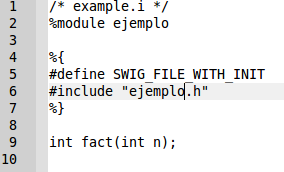
\includegraphics[scale=0.8]{Module_ejemplo.png}\\


La línea 5 inserta una macro que especifica que el archivo C resultante debe ser construido como una extensi\'on de Python, insertar el código de inicio del módulo. Este archivo i. envuelve el siguiente archivo C:

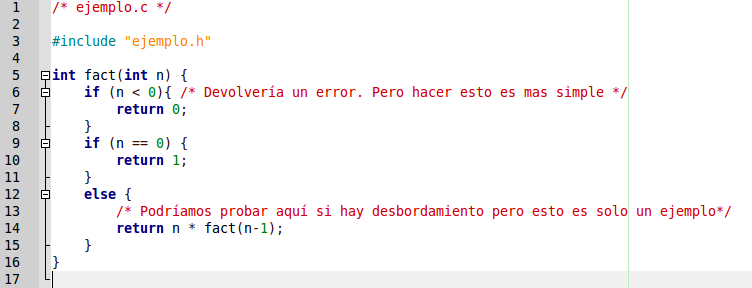
\includegraphics[scale=0.5]{ejemploC.png}\\

Con el archivo de cabecera:\\


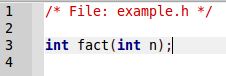
\includegraphics[scale=0.5]{ejemploH.png}\\

Para construir este modulo en Python usamos la opción "-python":\\

\textit{swig -python ejemplo.i}\\

Y si es la construcción de una extensión para C++, solo hay que añadir la opción "-c++":\\

\textit{swig -c++ -python ejemplo.i}\\


Esto crea dos archivos diferentes: uno \textit{ejemplo\_wrap.c}, o \textit{ejemplo\_wrap.cxx} si 
es de C++, y un archivo de origen \textit{example.py} Python
\textit{ejemplo\_wrap.c} es el archivo que se ha creado para la extensión. Estas funciones actúan como un pegamento entre los dos lenguajes. Ahora estos archivos los tenemos que compilar y un archivo con extension .so (archivos objeto), una vez creado esto, lo último que hay que hacer un enlace del archivo objeto:\\

Compilamos: \\

\textit{gcc -c ejemplo.c ejemplo\_wrap.c -I /usr/include/python2.7/}

Enlazamos los archivos .o para crear el archivo objeto de extensión .so, para no tener que volver a hacer estos pasos:\\

\textit{ld -shared ejemplo.o ejemplo\_wrap.o -o \_ejemplo.so}\\


Con esto estamos listos para usar el módulo que hemos creado en C para utilizarlo en Python.

Ejemplo:
\\

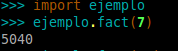
\includegraphics[scale=1]{ejemplo_fact.png}

\end{document}